
\item A \(2 \ \mu F\) capacitor is charged as shown in figure. The percentage of its stored energy dissipated after the switch \( S \) is turned to position \(2\) is
    \begin{center}
        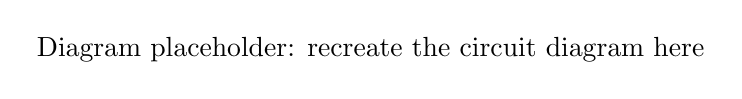
\begin{tikzpicture}
            % Since the actual diagram is not provided in text format, we put a placeholder comment here.
            % You should create the diagram based on the image provided.
            \node at (0, 0) {Diagram placeholder: recreate the circuit diagram here};
        \end{tikzpicture}
    \end{center}
    \begin{tasks}(2)
        \task \(0\%\)
        \task \(20\%\)
        \task \(75\%\)
        \task \(80\%\)
    \end{tasks}
